\documentclass[aps,reprint]{revtex4-1}
% Engine-specific settings
% Detect pdftex/xetex/luatex, and load appropriate font packages.
% This is inspired by the approach in the iftex package.
% pdftex:
\ifx\pdfmatch\undefined
\else
    \usepackage[T1]{fontenc}
    \usepackage[utf8]{inputenc}
\fi
% xetex:
\ifx\XeTeXinterchartoks\undefined
\else
    \usepackage{fontspec}
    \defaultfontfeatures{Ligatures=TeX}
\fi
% luatex:
\ifx\directlua\undefined
\else
    \usepackage{fontspec}
\fi
% End engine-specific settings
\usepackage[english]{babel}
\usepackage{csquotes}
% \usepackage[backend=biber, sortcites]{biblatex}
\usepackage{url}
\usepackage{textcomp}
\usepackage[usenames,dvipsnames,svgnames, table]{xcolor}
\usepackage[font={scriptsize}]{caption}
\usepackage{amsmath} \usepackage{amsthm} \usepackage{amsfonts}
\usepackage{amssymb}
\usepackage{enumerate}
\usepackage{tikz} \usepackage{float}
\usepackage[procnames]{listings}
\usepackage{pstool} \usepackage{pgfplots}
\usepackage{wrapfig} \usepackage{graphicx} \usepackage{epstopdf}
\usepackage{afterpage}
\usepackage{physics}
\usepackage{multirow}
\usepackage{gensymb}
\usepackage{algorithm}
\usepackage{microtype}
\usepackage[noend]{algpseudocode}
\usepackage{xcolor,colortbl}
\usepackage{microtype}
\usepackage{geometry}
\usepackage{hyperref}
\usepackage{graphicx}
\usepackage{caption}
\usepackage{subcaption}
\usepackage{lipsum}
% \usepackage{pythontex}
% \usepackage{authblk}
\usepackage{nth}
\usepackage{siunitx}
% \usepackage[toc,page]{appendix}
\floatstyle{plaintop}
\restylefloat{table}

% Custom commands
\newcommand{\unit}[1]{\:\mathrm{#1}}
\newcommand{\noref}[1]{\hyperref[#1]{\ref*{#1}}}
\newcommand{\nonref}[1]{\hyperref[]{\ref*{#1}}}
\newcommand\blankpage{%
  \null
  \thispagestyle{empty}%
  \addtocounter{page}{-1}%
  \newpage}

\newcommand{\mean}[1]{\langle #1 \rangle}

% Default fixed font does not support bold face
\DeclareFixedFont{\ttb}{T1}{txtt}{bx}{n}{7} % for bold
\DeclareFixedFont{\ttm}{T1}{txtt}{m}{n}{7}  % for normal

\newcommand\numberthis{\addtocounter{equation}{1}\tag{\theequation}}
\DeclareCaptionFont{white}{\color{white}}
\DeclareCaptionFormat{listing}{\colorbox{gray}{\parbox{\columnwidth}{#1#2#3}}}
\pgfplotsset{compat=1.14} %TODO: Setting this removed several error messages, should it be here!?


% Biber for references
% \bibliographystyle{aipauth4-1}

\begin{document}
\sisetup{detect-all}
\title{Ising (Or should I say Ezing?)}
\author{Erlend Lima}
\thanks{All code related to or referred by this paper was written in
  collaboration with Frederik J. Mellbye. This paper itself is written by
 solely the author.}
\affiliation{University of Oslo, Oslo, Norway \\ Source code available at: \url{https://github.com/Caronthir/FYS3150/tree/master/Project4}}
\date{\today}

\begin{abstract}
Once again the abstract abstractifies the abstractness of the abstract mathematical
equations than govern the universe.
\end{abstract}
\maketitle
\tableofcontents
\makeatletter
\let\toc@pre\relax
\let\toc@post\relax
\makeatother

\newpage

\section{Introduction}
\label{sec:introduction}

In his 1924 PhD thesis, Ernt Ising 
solved the one dimensional Ising model devised by his adviser, Wilhelm
Lenz~\cite{weicai}. Ising showed that no phase transition can occur in one
dimension, and so triumphantly declared that no phase transition can occur in
any dimension. Lars Onsager proved otherwise when he showed that there indeed
were phase transitions in two dimensions. Even though Ising was wrong, his name
is amongst the most common names in statistical mechanics. 
\section{Theory}
\label{sec:theory}

\subsection{The Ising Model}
\label{sec:isingmodel}

The Ising model is a microcanonical model which describes a lattice of discrete spins taking binary values, where each
spin interacts with its neighbors. Although simple, the Ising model is capable of modeling real
world phenomena such as ferromagnetism and phase transitions.

\begin{figure}[H]
  \centering
  \begin{tikzpicture}[thick]
    \draw[->] (0,0) -- (0,.3)  node [label=left:{$s_1$}] {};
    \draw[->] (1,0) -- (1,.3)  node [label=right:{$s_2$}] {};
    \draw[->] (0,1) -- (0,1.3) node [label=left:{$s_3$}] {};
    \draw[->] (1,1) -- (1,1.3) node [label=right:{$s_4$}] {};
    \draw[dotted] (-.75,-.4) rectangle (1.75,1.9);
  \end{tikzpicture}
  \caption{A two dimensional Ising model}
  \label{fig:22lattice}
\end{figure}
A lattice \(\Lambda\) is a \(d\)-dimensional graph with the nodes \(k\in\Lambda\) being spins
taking a discrete binary value, \(s_{k}\in\{-1, 1\}\). For a lattice of \(N\)
nodes, its energy is

\begin{equation}
  \label{eq:2}
 E = \sum_{<kl>}^{N}J_{k,l}s_{k}s_{l} - \sum_{k}^{N}\mathcal{B}_{k}s_{k}
\end{equation}

where \(<kl>\) denotes that the sum is taken over the neighboring spins.
Between any two spins \(k, l \in \Lambda\) there is an interaction \(J_{k,l}\),
and for any spin there is the possibility of an external magnetic field with
interaction \(\mathcal{B}_{k}\). Assuming that the spin interactions are equal
for all spins and the absence of an external magnetic field, the energy
simplifies to

\begin{equation}
  \label{eq:3}
  E = J\sum_{<kl>}^{N}s_{k}s_{l}
\end{equation}

For \(J>0\), it is favorable for neighboring spins to align, causing the
creation of magnetic domains throughout the lattice~\cite{physicslectures}.
This is called ferromagnetism. For \(J<0\), it is more favorable for spins to
point in opposite direction. The physical interpretation of this is
paramagnetism. In the remainder of this paper, it is assumed that \(J>0\).
The magnetism of the system is simply is sum over the spins,
\begin{equation}
  \label{eq:1}
  \mathcal{M} = \sum_{k} s_{k}
\end{equation}

Being microcanonical, the Ising model can be described by Boltzmann statistics.
Using this fact, it can be shown~\cite{physicslectures} that the heat capacity is
\begin{equation}
  \label{eq:4}
  C_V = \frac{\mean{E^2} - \mean{E}^2}{kT^2}
\end{equation}
and that the magnetic susceptibility is
\begin{equation}
  \label{eq:5}
  \chi = \frac{\mean{\mathcal{M}^2} - \mean{\mathcal{M}}^2}{kT}
\end{equation}
In addition, the first moment of energy can be written as
\begin{equation}
  \label{eq:6}
  \mean{E} = - \pdv{\ln{Z}}{\beta}
\end{equation}

\section{Method}
\label{sec:method}

\section{Results}
\label{sec:results}

\begin{figure}[ht]
  \centering
  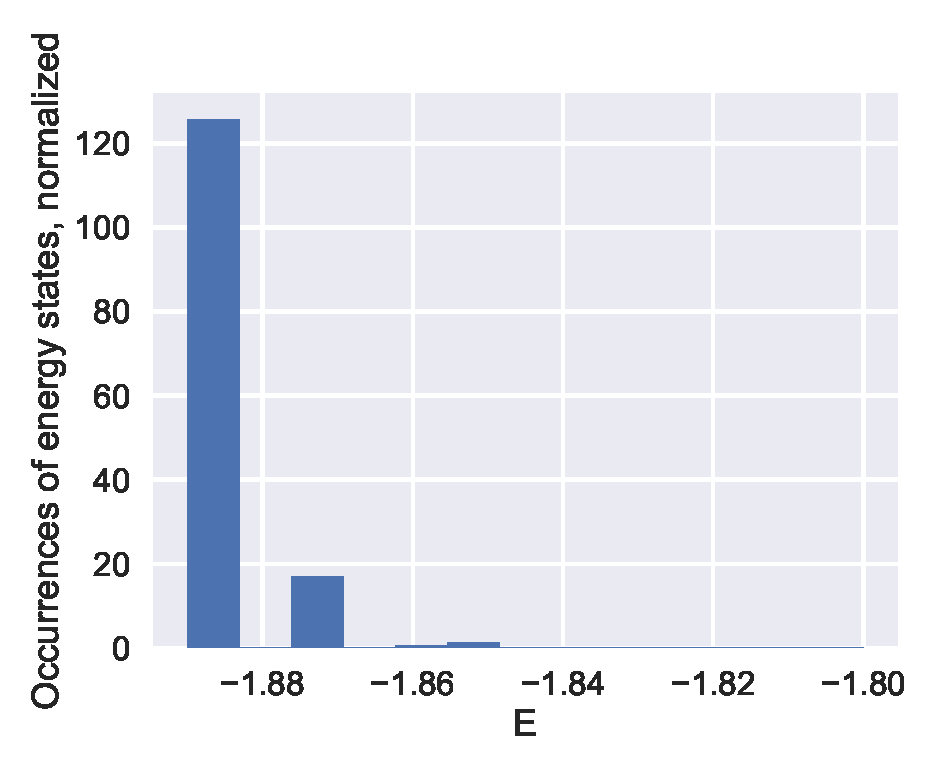
\includegraphics[width=\columnwidth]{figures/4da.eps}
  \caption{\label{fig:4da} Histogram over the energy states with \(T=1.0\) kT/J.
  The variance is \(\sigma^{2} \approx 5.845\cdot 10^{-5}\)}
\end{figure}

\begin{figure}[ht]
  \centering
  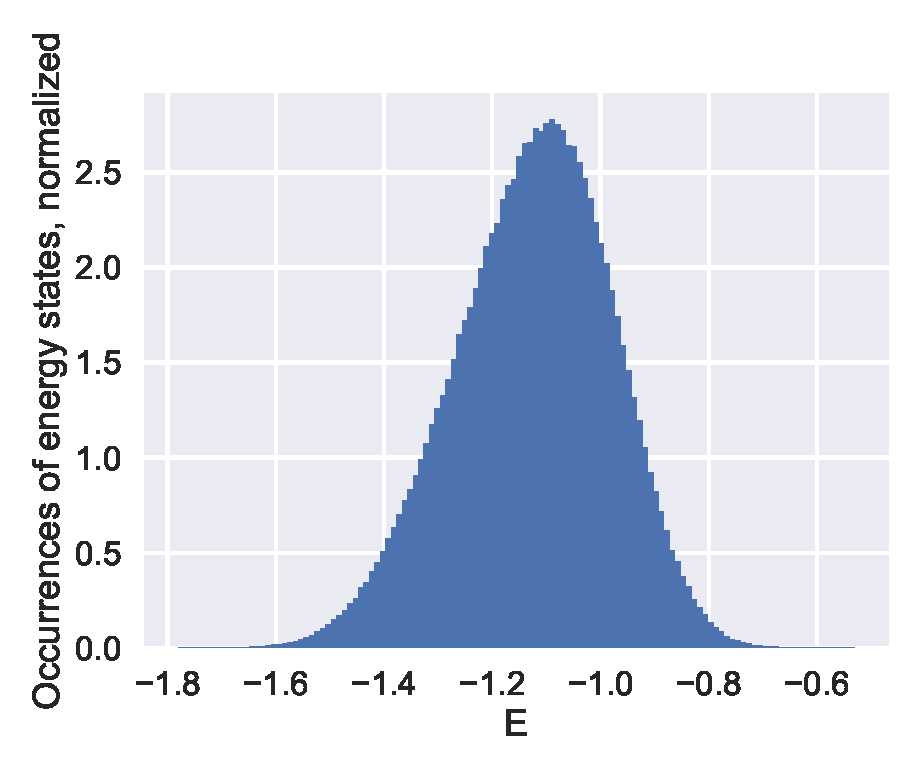
\includegraphics[width=\columnwidth]{figures/4db.eps}
  \caption{\label{fig:4db} Histogram over the energy states with \(T=2.4\) kT/J.
  The variance is \(\sigma^{2} \approx 0.0203\)}
\end{figure}

\section{Discussion}
\label{sec:discussion}

\section{Conclusion}
\label{sec:conclusion}

\bibliography{references}
\blankpage
\appendix
\section{Appending appendices is easy with the appendix package.}
\blankpage
\end{document}

% Local Variables:
% TeX-engine: luatex
% End:
